\begin{frame}
\frametitle{Is using Remy reasonable?}
\begin{itemize}
\item Training scenario:
\begin{tabular}{ll}
Link speed & 32 Mbits/sec \\
Minimum RTT & 150 ms \\
Topology & Dumbbell \\
Number of senders & 2 \\
Workload & 1 sec ON/OFF times \\
Buffer size & 5 BDP \\
Objective function & $\sum$ log(throughput) - log(delay)
\end{tabular}
\item Testing scenario identical to training scenario
\end{itemize}
\end{frame}

\begin{frame}
\frametitle{Is using Remy reasonable?}
\begin{itemize}
\item A hypothetical centralized scheme (CEN)
\begin{itemize}
\item Every time a sender turns ON/OFF, solve $\sum$ log (throughput)
\item Set each sender's rate using obtained solution
\item Zero queuing delay
\end{itemize}
\end{itemize}
\end{frame}

\begin{frame}
\frametitle{Is using Remy reasonable?}
\begin{centering}

\noindent \only<1>{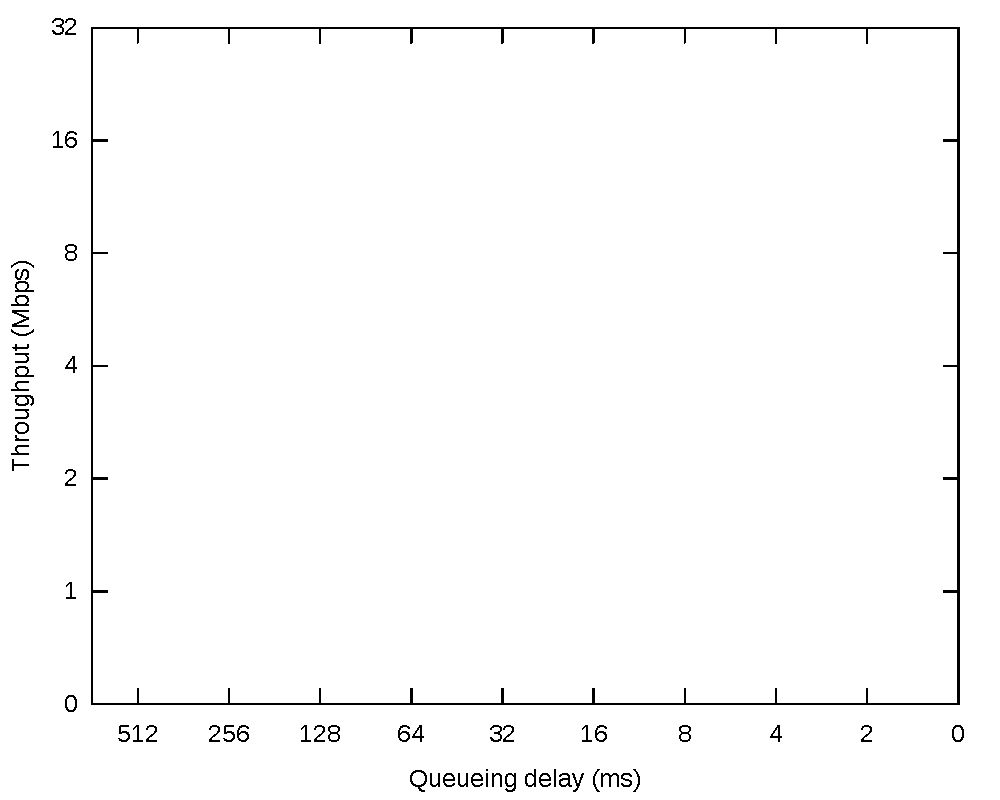
\includegraphics[width=3.3 in]{optimality-baseline.pdf}}\only<2>{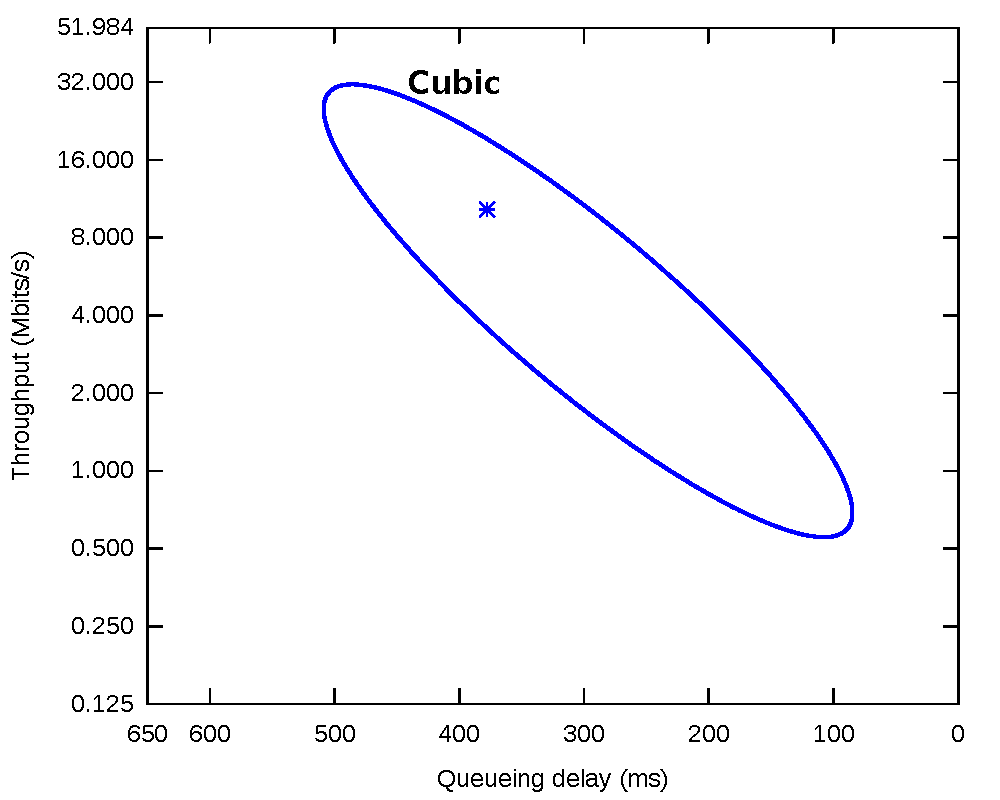
\includegraphics[width=3.3 in]{optimality-cubic.pdf}}\only<3>{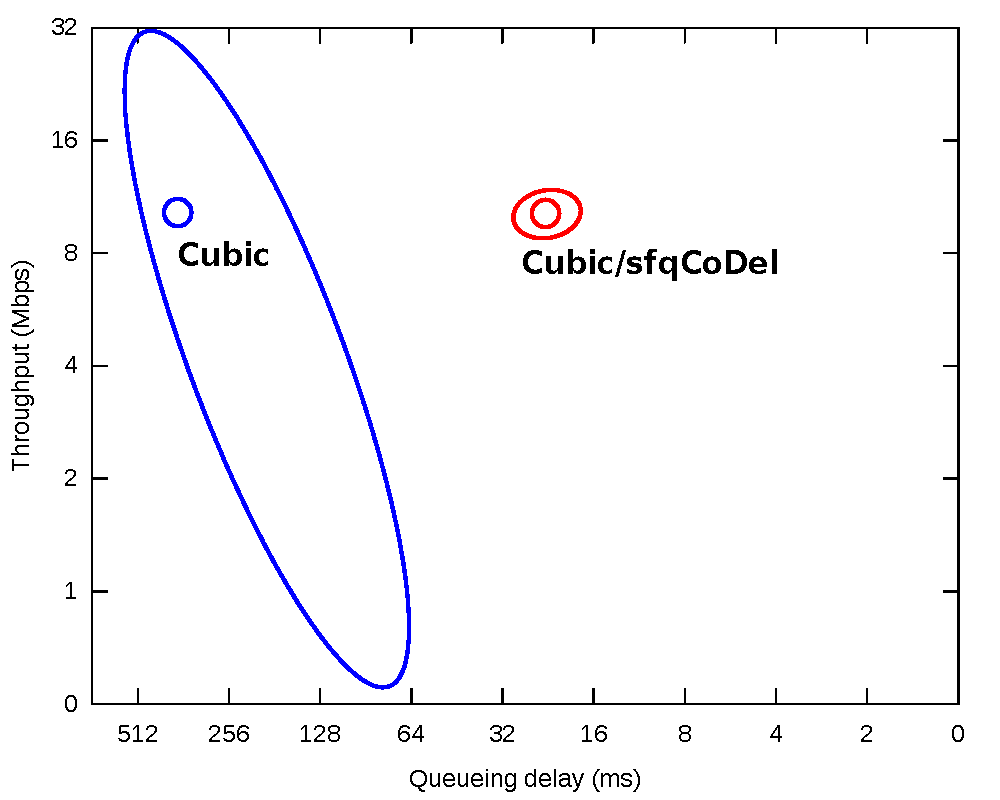
\includegraphics[width=3.3 in]{optimality-codel.pdf}}\only<4>{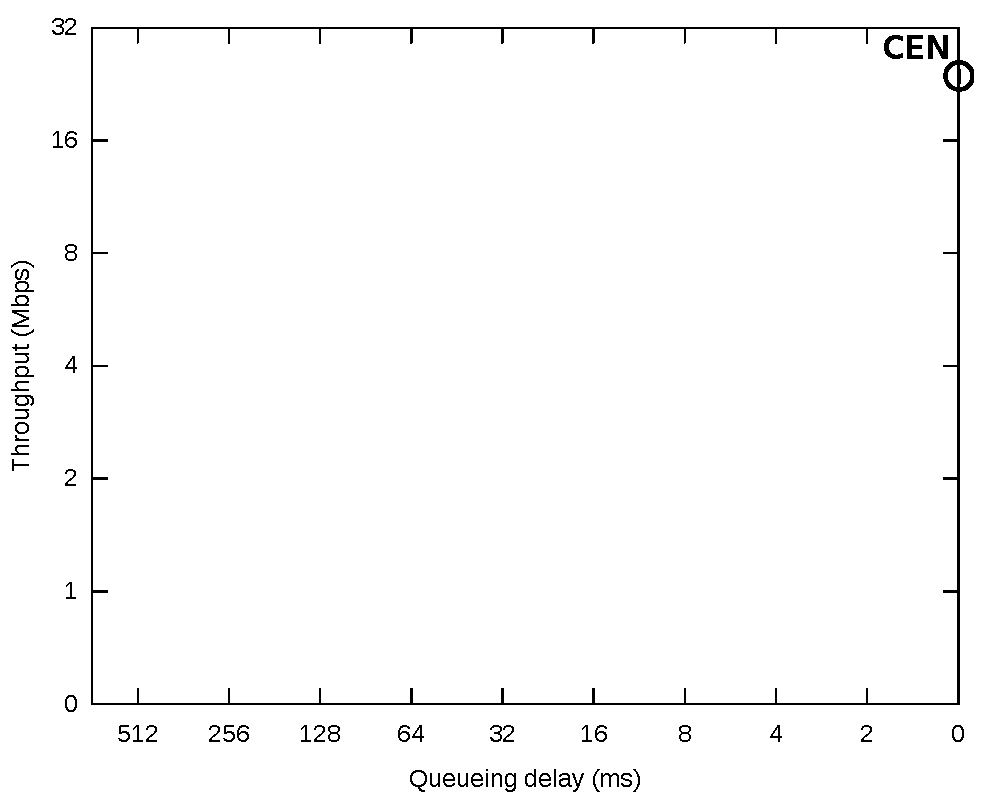
\includegraphics[width=3.3 in]{optimality-upper.pdf}}\only<5>{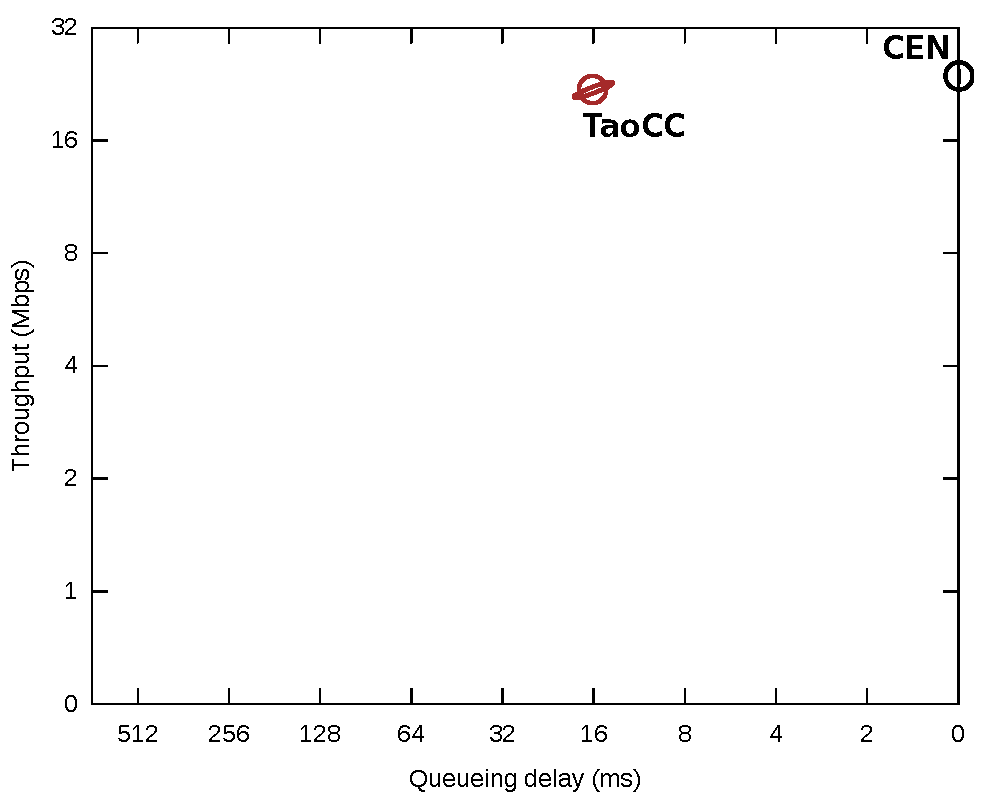
\includegraphics[width=3.3 in]{optimality-tao.pdf}}

\end{centering}
\end{frame}
